\documentclass{beamer}
\usepackage{beamerthemeshadow}
\usepackage[french]{babel}
\usepackage[T1]{fontenc}
\usepackage[utf8x]{inputenc}

\begin{document}
\title{Projet Puissance 4 en Java}  
\author{GAUTHIER Silvère}
\date{\today} 

\frame{\titlepage} 


\section{Slvr-Puissance 4}
\frame{\frametitle{Diagramme UML}

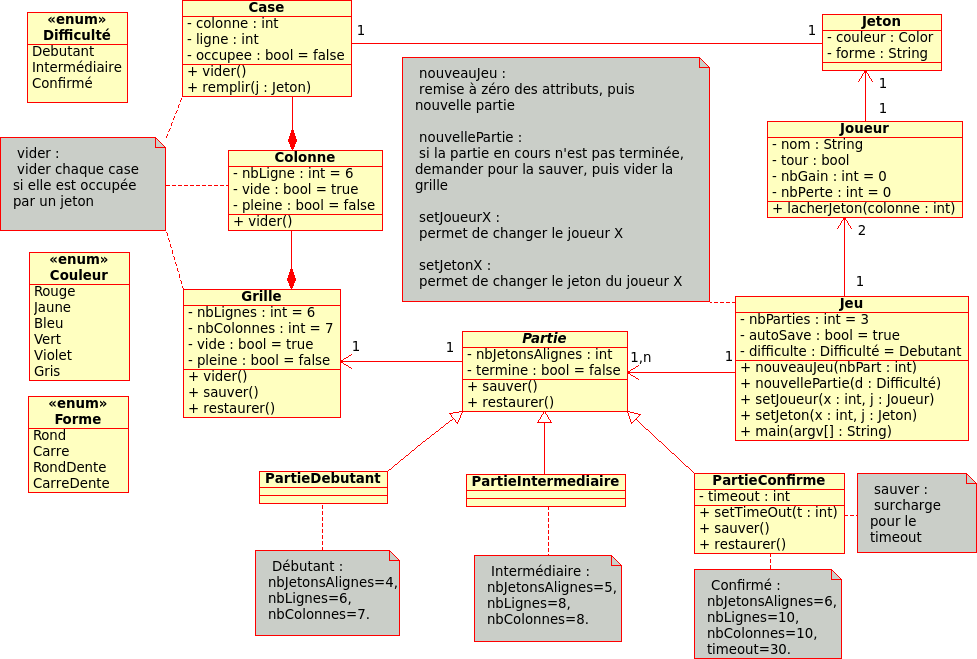
\includegraphics[scale=0.45]{DiagrammeModele.png}

}
\frame{\frametitle{Accueil}

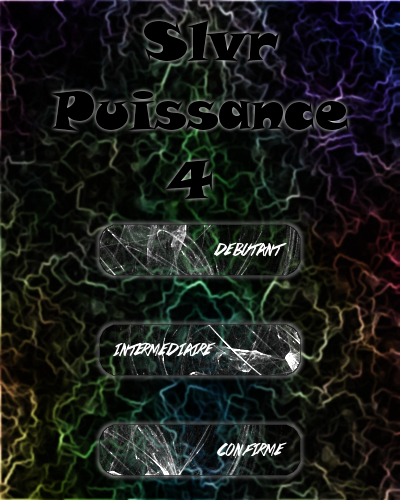
\includegraphics[scale=0.325]{FondAccueilFinal.png}

}
\frame{\frametitle{Jeu (Débutant)}

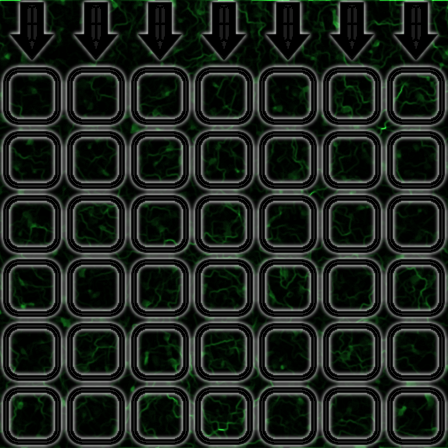
\includegraphics[scale=0.325]{DebutantFinal.png}

}
\frame{\frametitle{Jeu (Intermédiaire)}


\includegraphics[scale=0.325]{IntermediaireFinal.png}

}
\frame{\frametitle{Jeu (Confirmé)}

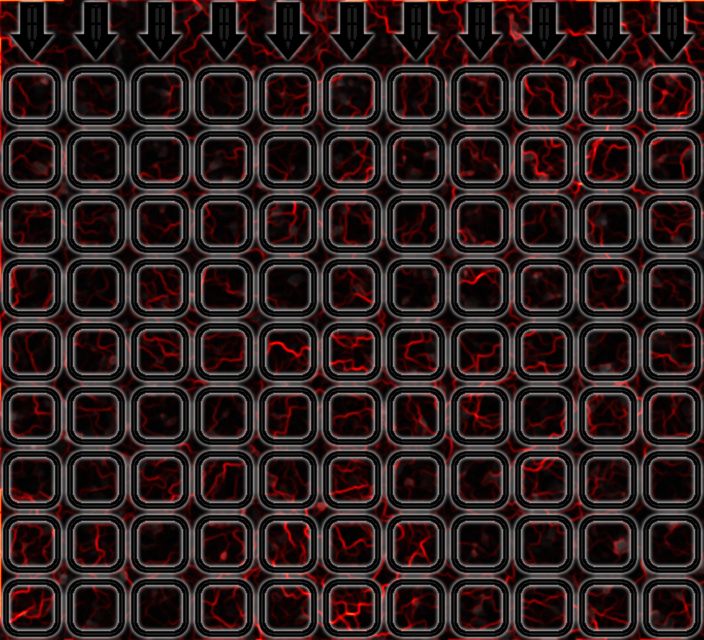
\includegraphics[scale=0.325]{ConfirmeFinal.png}

}
\frame{\frametitle{Jeu (Exemple)}

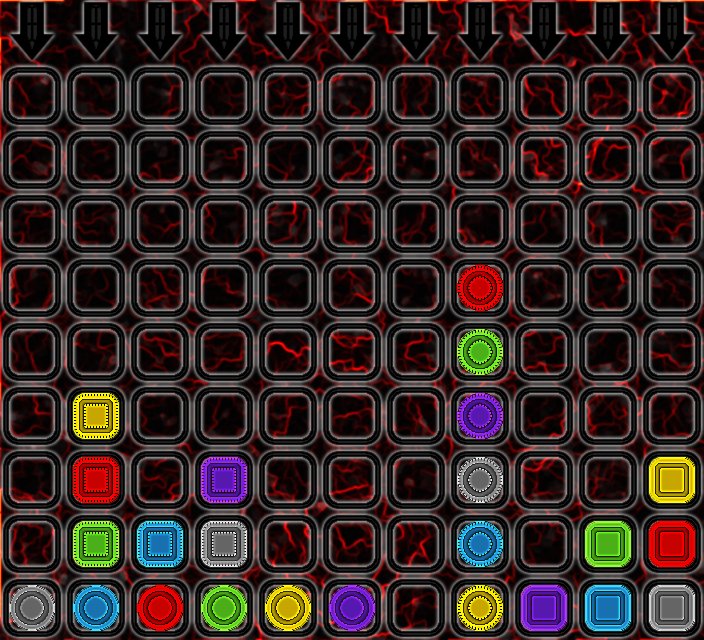
\includegraphics[scale=0.325]{sample.png}

}
\end{document}

